% Systemdokumentation OOP3
% Unterlage für Studenten als Leitfaden für die Erstellung einer SystemDoku
% 17. Oktober 2022
% ---------------------------------------------------------------------------



% Dokumentklasse
% --------------
\documentclass[12pt,naustrian,a4widepaper]{scrartcl}   
% article style
%   - 11pt Schriftgroesse
%   - new austrian (neue Rechtschreibung)
%   - Papierformat A4
%   - pdf-hyperlinks


% Packages
% --------
\usepackage[utf8]{inputenc}  % fuer Umlaute, Ü
\usepackage[T1]{fontenc}
\usepackage{a4wide}
\usepackage{times}      % Times Schriften (zusammen mit fontencoding, s.o.)

\usepackage{babel}
\usepackage{graphicx}	  % für das Einbinden von Grafiken
\usepackage{color}      % für färbigen Text
\usepackage{framed}     % für (Text-) Rahmen
\usepackage{fancyhdr}   % für Kopf- und Fusszeilen
\usepackage{listings}   % für den Sourcecode
\usepackage{pdfpages}

\pagestyle{fancy}       % Kopf- / Fusszeile aktivieren

\definecolor{failred}{rgb}{0.7, 0.0, 0.0}
\definecolor{okgreen}{rgb}{0.0, 0.5, 0.0}
\definecolor{gray}{rgb}{0.0, 0.5, 0.0}

\lstdefinelanguage{TestOutput}{
    morekeywords={},
    morecomment=[l]{//},
    morestring=[b]",
    sensitive=false,
}

\lstdefinestyle{teststyle}{
    language=TestOutput,
    basicstyle=\ttfamily\footnotesize,
    keywordstyle=\color{black},
    commentstyle=\color{gray},
    stringstyle=\color{black},
    showstringspaces=false,
    breaklines=true,
    frame=single,
    numbers=left,
    numberstyle=\tiny\color{gray},
    postbreak=\mbox{\textcolor{red}{$\hookrightarrow$}\space},
    literate={OK}{{\textcolor{okgreen}{OK}}}2
             {Fail}{{\textcolor{failred}{Fail}}}4,
}

\lstset{
	language={C++},
	basicstyle=\tiny\ttfamily,
	keywordstyle=\color{blue},%\bfseries,
	commentstyle=\color{green},
	frame=single,
	linewidth=16cm,
	breaklines=false,
	tabsize=3,
	numbers=left, numberstyle=\tiny, stepnumber=1, numbersep=5pt
}


% Seitenspiegel
% -------------

\typearea{8}	% Festlegung des Seitenspiegels gem. Koma. 4..groß, 9..klein


% Kopfzeile
% ---------
\lhead{{\footnotesize{s. Offenberger, S. Vogelhuber}}}   %  (links)
\chead{{\footnotesize{Systemdokumentation - Fuhrpark}}} %  (mitte)
\rhead{{\footnotesize{Seite \thepage}}}      %  (rechts)

% Fusszeile
% ---------
\lfoot{}  % links
\cfoot{}  % mitte 
\rfoot{}  % rechts

% Absatzformatierung
% ------------------
\setlength{\parindent}{0cm}   % Einrückung der 1. Zeile jedes Absatzes
\setlength{\parskip}{10pt}    % Abstand zwischen den Absätzen


% Package für Hyperlinks (mit pdf-Optionen)
% -----------------------------------------
\usepackage[
urlcolor=blue,		% blaue weblinks
linkcolor=black,	% interne Links sind schwarz
colorlinks=true,        % links werden eingefärbt
pdfstartview=FitH,      % PDF-Anzeige: Fensterbreite
pdfborder={0 0 0},      % keine Umrandung um links
pdftitle   ={Systemdokumentation},% Referenzen in der Pdf-Datei
pdfauthor  ={M. Mustermann, S. Sorglos},
pdfsubject ={Systemdoku},
pdfcreator ={Der Creator},
pdfproducer={Der Producer},
pdfkeywords={Dokumentation, Systemdokumentation}
]{hyperref}


% Beginn des Dokumentes
% ---------------------
\begin{document}

\selectlanguage{naustrian}   % oder "american" für engl. Texte

% Titelblatt
% ----------
\title {\vspace{1cm}
       
\includegraphics[width=8cm]{./Images/FhOOeLogoOkt2009_HSD_Rot_pastell}\\
       \vspace{2cm}
       {\textbf{Systemdokumentation\\Projekt Gehaltsberechnung}}\\
       \vspace{5mm}
       {\small{Version 1.0}}\\
       \vspace{5mm}
}

\author{\small{S. Offenberger, S. Vogelhuber}}
\date  {\small{Hagenberg, \today}}
\maketitle

%\begin{abstract}
%Dieses Dokument zeigt den prinzipiellen Aufbau einer Systemdokumentation für Software-Projekte. Die einzelnen Kapitel sind mit Kommentaren versehen, welche die Struktur und den Inhalt erläutern. 
%\end{abstract}

\clearpage

% Inhalts-, Tabellen- und Bildverzeichnis (werden generiert)
% ----------------------------------------------------------
\tableofcontents
% \listoftables
% \listoffigures
\clearpage



\section{Organisatorisches}

\subsection{Team}
\begin{itemize}
	\item Simon Offenberger, Matr.-Nr.: S2410306027, E-Mail: Simon.Offenberger@fh-hagenberg.at
	\item Simon Vogelhuber, Matr.-Nr.: S2410306014, E-Mail: s2410306014@fhooe.at	
\end{itemize}

\subsection{Aufteilung der Verantwortlichkeitsbereiche}
\begin{itemize}
	\item Simon Offenberger
		\begin{itemize}
			\item Design Klassendiagramm
			\item Implementierung und Test der Klassen: 
			\begin{itemize}
				\item Company
				\item Company Interface
				\item Client
			\end{itemize}
			\item Implementierung des Testtreibers
			\item Dokumentation
		\end{itemize}
	\item Simon Vogelhuber
		\begin{itemize}
			\item Design Klassendiagramm
			\item Implementierung und Komponententest der Klassen: 
			\begin{itemize}
				\item Employee
				\item Boss
				\item ComissionWorker
				\item PieceWorker
				\item HourlyWorker
			\end{itemize}
			\item Implementierung des Testtreibers
			\item Dokumentation
		\end{itemize}	
\end{itemize}

\subsection{Aufwand}
	
	\begin{itemize}
		\item Simon Offenberger: geschätzt 10 Ph / tatsächlich x Ph
		\item Simon Vogelhuber:  geschätzt x Ph / tatsächlich x Ph
	\end{itemize}

\clearpage
\section{Anforderungsdefinition (Systemspezifikation)}
In diesem Projekt geht es darum die Mitarbeiter eines Unternehmens zu verwalten und deren Gehälter zu berechnen.
Es gibt verschiedene Arten von Mitarbeitern, welche unterschiedliche Gehaltsberechnungen haben. Der Zugriff 
auf die Mitarbeiter soll über eine gemeinsame Schnittstelle erfolgen.
\\
\\
\textbf{Funktionen der Firmenschnittstelle}
\begin{itemize}
	\item Zugriff auf die wichtigsten Mitarbeiter und Firmendaten
\end{itemize}

\textbf{Funktionen der Firma}
\begin{itemize}
	\item Verwalten von Mitabeitern verschiedener Arten.
	\item Ausgabe von Firmen und Mitarbeiterinformationen.
	\item Anlegen und Entfernen von Mitarbeitern.
\end{itemize}

\textbf{Funktionen der Mitarbeiter}
\begin{itemize}
	\item Speichern von Mitarbeiterdaten.
	\item Berechnung des Gehalts.
	\item Ausgabe von Mitarbeiterinformationen.
\end{itemize}

\clearpage
\section{Systementwurf}

\subsection{Klassendiagramm}
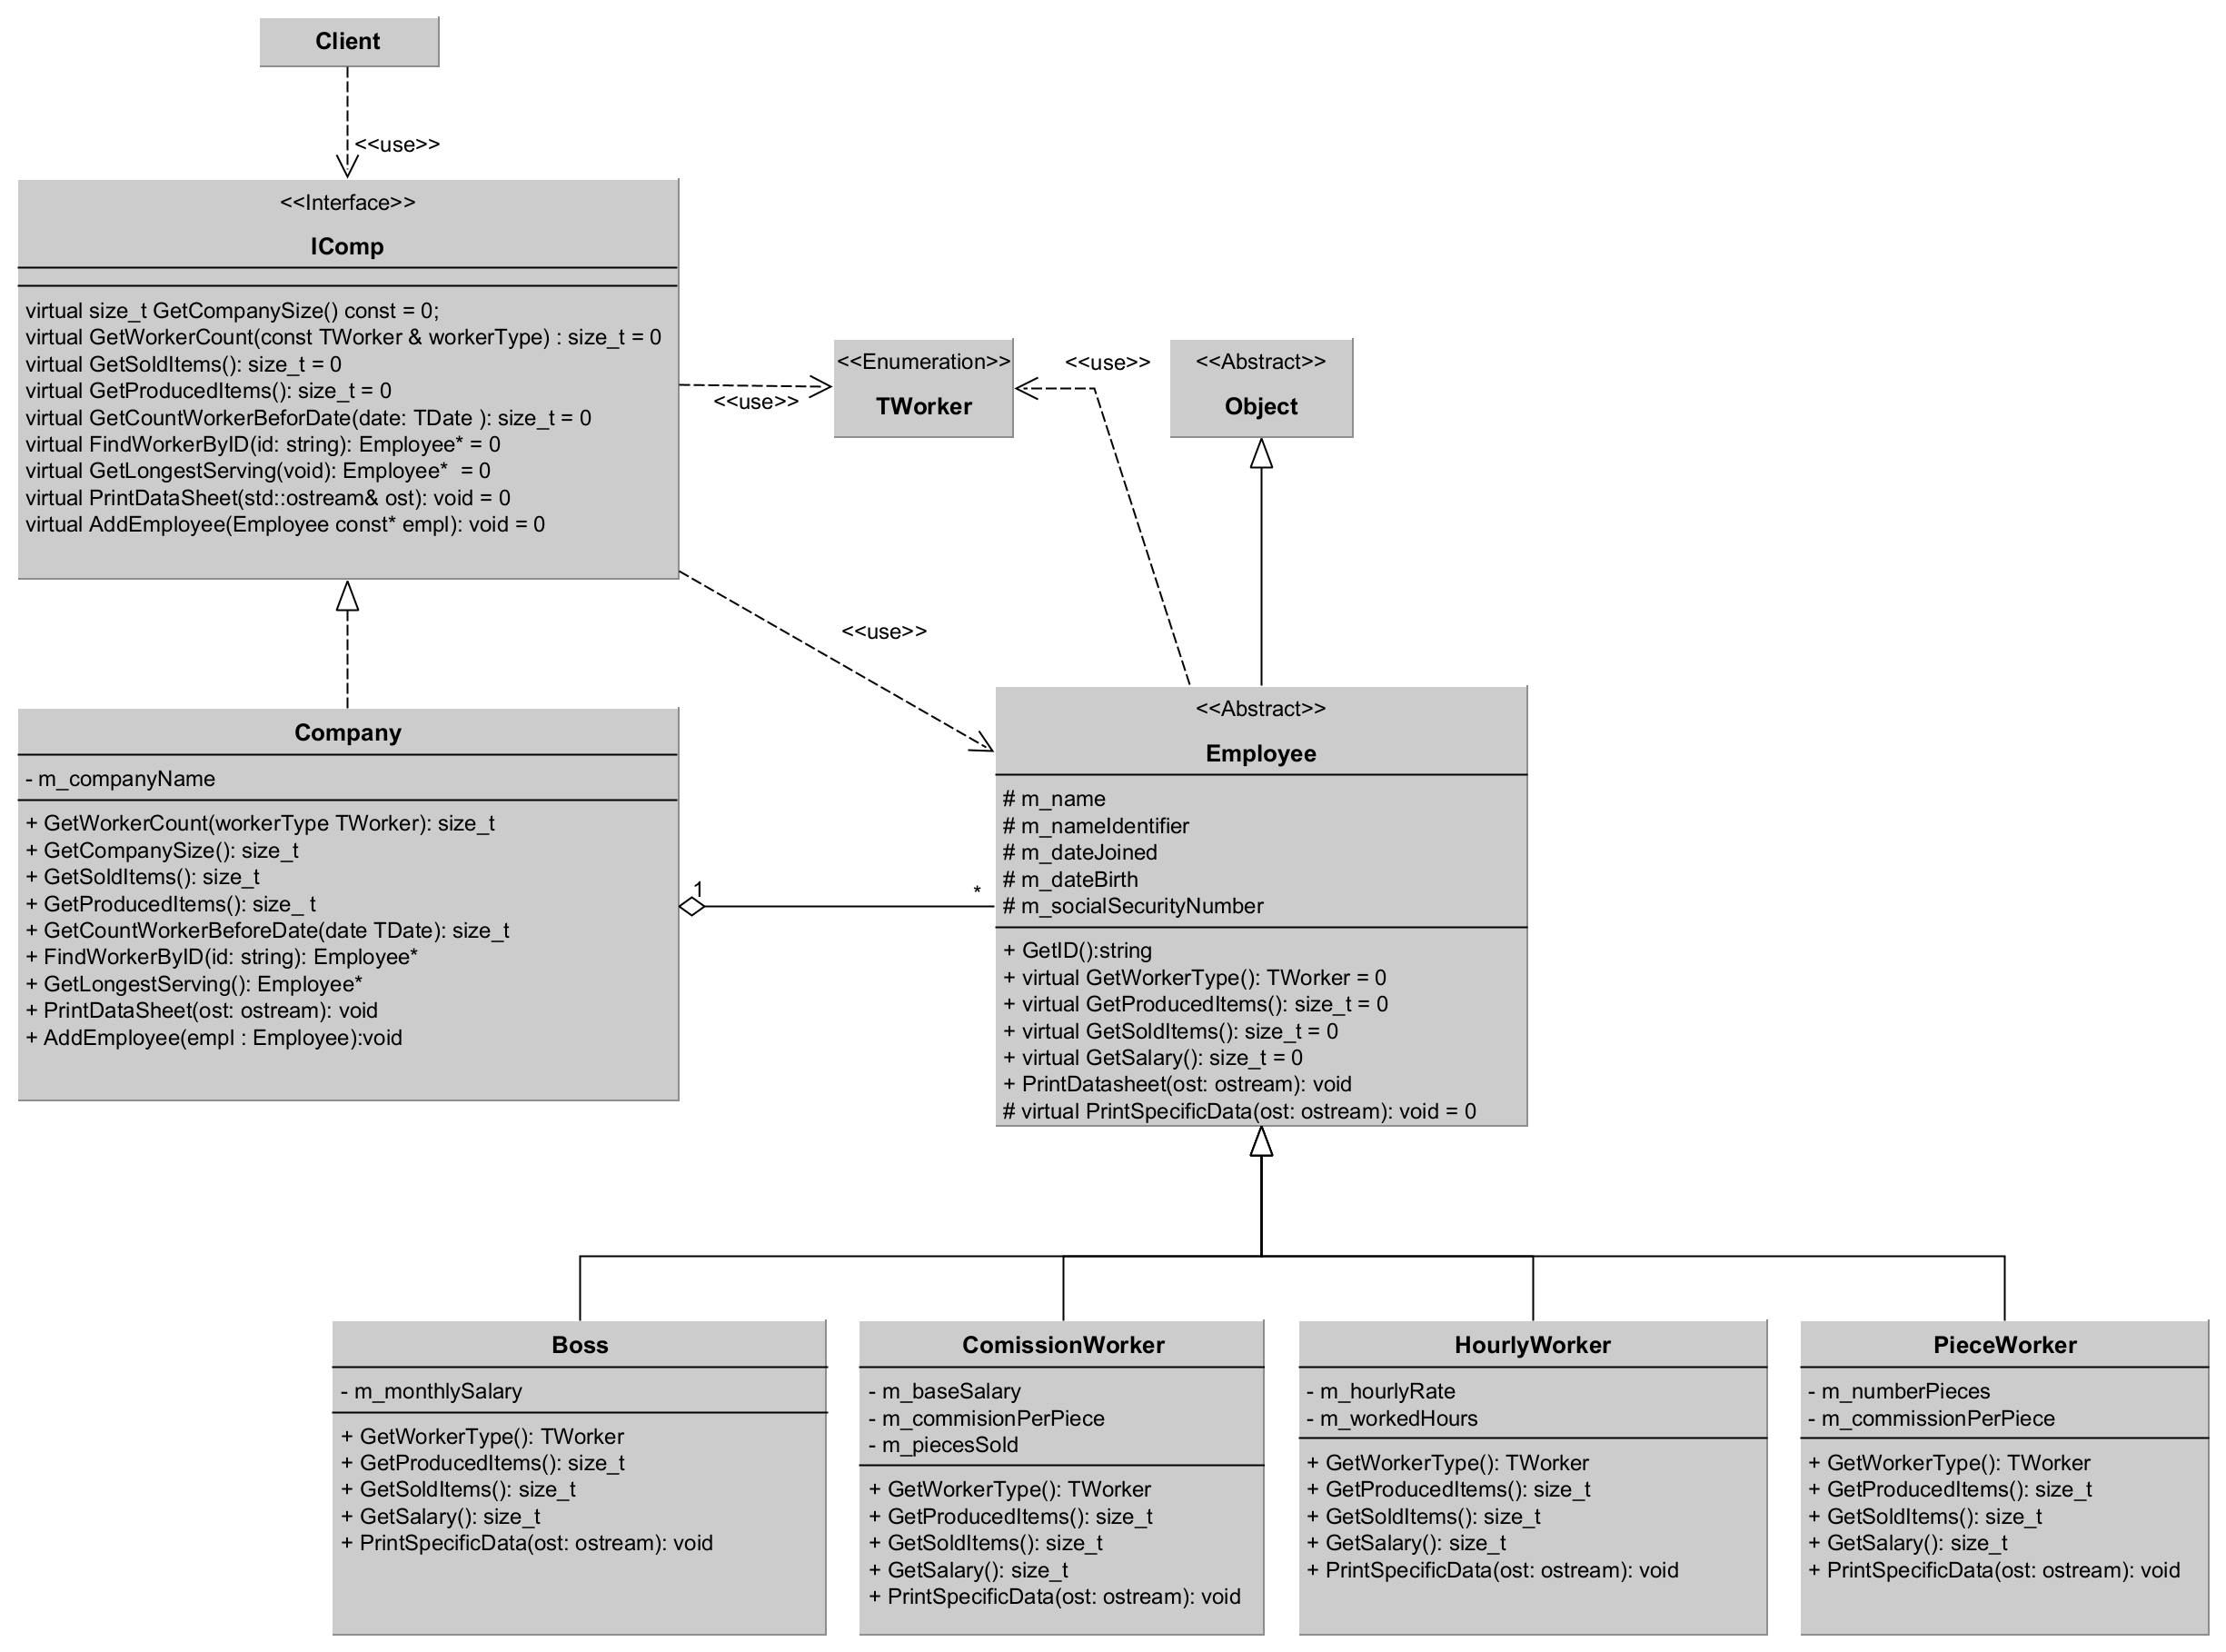
\includegraphics[width=14cm]{./Images/UML_Diagramm.png}
\newpage

\subsection{Designentscheidungen}

Das Interface \textbf{ICompany} wurde erstellt, um dem zugreifenden \textbf{Client} eine Schnittstelle zur Verfügung zu stellen.
Dadurch kann sich der Client auf die Schnittstelle konzentrieren und muss sich nicht um die Implementierungsdetails der Firma kümmern.
\\
\\
Die Firma ist ein polymorpher Container, der Objekte der abstrakten Klasse \textbf{Employee} verwaltet.
Bei dem Container wurde eine Map verwendet, da die Mitarbeiter über eine eindeutige ID angesprochen werden können.
\\
\\
Die Klasse \textbf{Employee} ist abstrakt, da es keine generellen Mitarbeiter geben soll, sondern nur spezielle Arten von Mitarbeitern.
Die einzelnen Mitarbeiter speichern Daten, die für die Gehaltsberechnung notwendig sind. 
Die Gehaltsberechnung wird über eine virtuelle Funktion realisiert, die in den abgeleiteten Klassen überschrieben wird.
\\
\\
Das Enum mit dem Mitarbeitertypen \textbf{TWorker} wurde eingebaut, da die Company den Typen des Mitarbeiters kennen muss, um den Mitarbeiter korrekt anzulegen.
Hierbei wurde aktiv auf RTTI verzichtet, um die Kopplung zwischen Company und Employee zu reduzieren.

\color{black}

\section{Dokumentation der Komponenten (Klassen)}
Die HTML-Startdatei befindet sich im Verzeichnis \href{run:./../doxy/html/index.html}{./../doxy/html/index.html}


\clearpage
\section{Testprotokollierung}
%\lstinputlisting[style=teststyle]{../TestOutput.txt}

\clearpage
\section{Quellcode}

\subsection{Object.hpp}
\lstinputlisting{../Object.hpp}

\subsection{Client.hpp}
\lstinputlisting{../Client.hpp}
\subsection{Client.cpp}
\lstinputlisting{../Client.cpp}

\subsection{IComp.hpp}
\lstinputlisting{../IComp.hpp}

\subsection{Company.hpp}
\lstinputlisting{../Company.hpp}
\subsection{Company.cpp}
\lstinputlisting{../Company.cpp}

\subsection{TWorker.hpp}
\lstinputlisting{../TWorker.hpp}

\subsection{Employee.hpp}
\lstinputlisting{../Employee.hpp}
\subsection{Employee.cpp}
\lstinputlisting{../Employee.cpp}

\subsection{Boss.hpp}
\lstinputlisting{../Boss.hpp}
\subsection{Boss.cpp}
\lstinputlisting{../Boss.cpp}

\subsection{HourlyWorker.hpp}
\lstinputlisting{../HourlyWorker.hpp}
\subsection{HourlyWorker.cpp}
\lstinputlisting{../HourlyWorker.cpp}

\subsection{PieceWorker.hpp}
\lstinputlisting{../PieceWorker.hpp}
\subsection{PieceWorker.cpp}
\lstinputlisting{../PieceWorker.cpp}

\subsection{ComissionWorker.hpp}
\lstinputlisting{../ComissionWorker.hpp}
\subsection{ComissionWorker.cpp}
\lstinputlisting{../ComissionWorker.cpp}

\subsection{main.cpp}
\lstinputlisting{../main.cpp}

% Literaturverzeichnis
% --------------------
%\begin{thebibliography}{99}
%\bibitem{Pomberger} Pomberger G., Blaschek G. : \textit{Software Engineering: Prototyping und objektorientert Software-Entwicklung}. Hanser, 1996
%
%\end{thebibliography}


% Ende des Dokuments
% ------------------
\end{document}
